% $File: report.tex
% $Date: Sun Dec 23 01:42:52 2012 +0800
% $Author: wyx <ppwwyyxxc@gmail.com>

\documentclass[a4paper]{article}
\usepackage{fontspec,zhspacing,verbatim,minted, zhmath}
\usepackage{amsmath}
\usepackage[hyperfootnotes=false,colorlinks,linkcolor=blue,anchorcolor=blue,citecolor=blue]{hyperref}
\usepackage{amssymb,amsthm,fontspec,graphicx,algpseudocode}
%\usepackage[sorting=none]{biblatex}
\usepackage{cite}
\usepackage{subfigure}
\usepackage{textcomp,enumerate}
\usepackage{indentfirst}
\usepackage{float,chngpage}
\usepackage{titlesec}
\usepackage{fancyhdr}
\usepackage{extarrows}
\usepackage{titlesec}
\usepackage{caption}\captionsetup{hypcap=true}
\usepackage{indentfirst}
\newfontfamily\zhfont[BoldFont=SimHei,ItalicFont=KaiTi_GB2312]{SimSun}
\zhspacing


\changetext{}{2.2cm}{-1.1cm}{-1.1cm}{}
\pagestyle{fancy}
\setlength{\headheight}{15.2pt}
\lhead[]{}\rhead[]{}
%\chead[\em 探究人耳对语言的辨识]{\em 探究人耳对语言的辨识}
\fancyhead[C]{\emph{Number of Fixed Points in Random Permutations}}

%\renewcommand{\abstractname}{摘要}
%\renewcommand{\contentsname}{目录}
%\renewcommand{\figurename}{图}
%\defbibheading{bibliography}{\section{References}}

\newcommand{\figref}[1]{\hyperref[fig:#1]{Figure \ref*{fig:#1}}}
\newcommand{\eqnref}[1]{\hyperref[eqn:#1]{(\ref*{eqn:#1})}}
\newcommand{\lemref}[1]{\hyperref[lemma:#1]{Lemma \ref*{lemma:#1}}}
\newcommand{\secref}[1]{\hyperref[sec:#1]{Section \ref*{sec:#1}}}
\DeclareMathOperator{\LM}{\tiny{LM}}
\DeclareMathOperator{\LT}{\tiny{LT}}
\DeclareMathOperator{\rank}{\tiny{rank}}
\DeclareMathOperator{\sgn}{sgn}
\DeclareMathOperator{\Cov}{Cov}

\let\Oldsum\sum
\renewcommand{\sum}{\displaystyle\Oldsum}
\let\Oldprod\prod
\renewcommand{\prod}{\displaystyle\Oldprod}
\let\Oldcap\bigcap
\renewcommand{\bigcap}{\displaystyle\Oldcap}
\let\Oldcup\bigcup
\renewcommand{\bigcup}{\displaystyle\Oldcup}
\let\Oldint\int
\renewcommand{\int}{\displaystyle\Oldint}
\let\Oldiint\iint
\renewcommand{\iint}{\displaystyle\Oldiint}

% $File: mint-defs.tex
% $Date: Sat Feb 16 22:59:11 2013 +0800
% $Author: wyx <ppwwyyxxc@gmail.com>

\usepackage{xparse}


% \inputmintedConfigured[additional minted options]{lang}{file path}{
\newcommand{\inputmintedConfigured}[3][]{\inputminted[fontsize=\footnotesize,
	label=#3,linenos,frame=lines,framesep=0.8em,tabsize=4,#1]{#2}{#3}}

% \phpsrc[additional minted options]{file path}: show highlighted php source
\newcommand{\phpsrc}[2][]{\inputmintedConfigured[#1]{php}{#2}}
% \phpsrcpart[additional minted options]{file path}{first line}{last line}: show part of highlighted php source
\newcommand{\phpsrcpart}[4][]{\phpsrc[firstline=#3,firstnumber=#3,lastline=#4,#1]{#2}}
% \phpsrceg{example id}
\newcommand{\phpeg}[1]{\inputminted[startinline,
	firstline=2,lastline=2]{php}{res/php-src-eg/#1.php}}

\newcommand{\txtsrc}[2][]{\inputmintedConfigured[#1]{text}{#2}}
\newcommand{\txtsrcpart}[4][]{\txtsrc[firstline=#3,firstnumber=#3,lastline=#4,#1]{#2}}

\newcommand{\pysrc}[2][]{\inputmintedConfigured[#1]{py}{#2}}
\newcommand{\pysrcpart}[4][]{\pysrc[firstline=#3,firstnumber=#3,lastline=#4,#1]{#2}}

\newcommand{\confsrc}[2][]{\inputmintedConfigured[#1]{squidconf}{#2}}
\newcommand{\confsrcpart}[4][]{\confsrc[firstline=#3,firstnumber=#3,lastline=#4,#1]{#2}}

\newcommand{\cppsrc}[2][]{\inputmintedConfigured[#1]{cpp}{#2}}
\newcommand{\cppsrcpart}[4][]{\cppsrc[firstline=#3,firstnumber=#3,lastline=#4,#1]{#2}}

\renewcommand{\P}[1]{\text{P}\left(#1\right)}
\renewcommand{\Pr}[1]{\text{Pr}\left\{#1\right\}}
\newcommand{\Px}[2]{\text{P}_{#1}\left(#2\right)}
\newcommand{\E}[1]{\text{E}\left[#1\right]}
\newcommand{\Ex}[1]{\text{E}#1}
\newcommand{\Var}[1]{\text{Var}\left[#1\right]}
%\newcommand{\Cov}[2]{\text{Cov}\left[#1,#2\right]}
%\newcommand{\Cov}[1]{\text{Cov}\left[#1 \right]}
\renewcommand{\T}[1]{\Theta\left(#1\right)}
\newcommand{\real}{\mathbb{R}}
\newcommand{\card}[1]{\left\|#1\right\|}
\newtheorem{lemma}{Lemma}

\NewDocumentCommand\Cov{mg}{
    \text{Cov}\left[ #1 \IfNoValueTF{#2}{}{,#2}\right]
 }

\newcommand{\qed}{\hfill \ensuremath{\Box}}



\title{Number of Fixed Points in Random Permutations}
\author{Yuxin Wu~(2011011271)\\Dept. of Computer Science and Technology, Tsinghua Univ.\\<ppwwyyxxc@gmail.com>}
\date{Dec. 2012}

\begin{document}
\maketitle
\begin{abstract}
  In this paper, we will focus on various features of the random variable $X$
  defined by the number of fixed points in random permutations.
  The distribution of $X$ will be given in several forms, an approximate distribution will be discussed.
  The moments as well as the generating functions of $X$ will also be calculated.

  \textbf{Keywords:} random permutations, dearrangements, fixed points, rencontres numbers
\end{abstract}
\tableofcontents
\newpage
% $File: notation.tex
% $Date: Sun Dec 23 01:04:29 2012 +0800
% $Author: jiakai <jia.kai66@gmail.com>

\section*{Notations}
Throughout this paper, we would use the following notations:
\begin{itemize}
	\item $\Pr{S}$ is the probability of $S$ ($S$ is usually a set or a
		proposition).
	%\item $\Px{X}{x}$ is the probability distribution function for random
		%variable $X$, and if $X$ is discrete we have $\Px{X}{x} = \Pr{X = x}$.
		%We would write $\P{x}$ instead of $\Px{X}{x}$ if there is no ambiguity.
	\item $\E{X}$ is the expectation of random variable $X$, which is defined
		as the following for a discrete random variable:
		\begin{equation*}
			\E{X} = \sum_k k\P{k}
		\end{equation*}
	\item $\Var{X}$ is the variance of random variable $X$, defined as
		\begin{equation*}
			\Var{X} = \E{(X-\E{X})^2}
		\end{equation*}
	\item $\Cov[X,Y]$ is the covariance of random variables $X, Y$, defined as
		\begin{equation*}
			\Cov[X,Y] = \E{XY}-\E{X}\E{Y}
		\end{equation*}
	%\item $\T{f(n)}$ and $\O{f(n)}$ are used to describe the asymptotic behavior
		%of functions, defined as:
		%\begin{quote}
			%$f(n) = \O{g(n)}$ iff $\exists N_0, c \in \real$ such that
			%\begin{equation*}
				%\forall n > N_0, |f(n)| < c|g(n)|
			%\end{equation*}
			%$f(n) = \T{g(n)}$ iff $f(n) = \O{g(n)}$ and $g(n) = \O{f(n)}$
		%\end{quote}
\end{itemize}

% vim: filetype=tex foldmethod=marker foldmarker=f{{{,f}}}


% File: intro.tex
% Date: Wed Jul 17 14:44:12 2013 +0800
% Author: Yuxin Wu <ppwwyyxxc@gmail.com>

\section{Introduction}
Let $ \pi= (\pi(1), \pi(2),\cdots ,\pi(n))$ be a permutation of $ (1,2,\cdots ,n)$.
The \emph{Fixed Points} of the permutation $ \pi$ ,
denoted as $ \mathcal{F}(\pi)$, is defined as follows:
\[ \mathcal{F}(\pi) = \{ k \in [1,n]\cap \mathbb{N} \mid \pi(k) = k \}\]

Let $ \Pi_n$ be the set of all possible permutations of $ (1,2,\cdots ,n)$.
The \emph{Rencontres Numbers}\cite{wiki_rn}
$ D_{n,k}$ is defined as follows:
\[ D_{n,k} = \card{ \{ \pi \in \Pi_n \mid \card{\mathcal{F}(\pi)} = k \}}, k = 0,1,\cdots n\]
where $ \card{A}$ is the cardinality of a set $ A$.

In particular, we denote $ D_{n,0}$ as $  D_{n} $ for short.

Let $ \pi $ be a random permutation of $ (1,2,\cdots ,n),$ where
every possible permutation has the same possibility $ \dfrac{1}{n!}$.
The random variable $ X = \card {\mathcal{F}(\pi)} $ is what we will focus on in this paper.


% File: cal_d.tex
% Date: Sun Dec 23 15:39:45 2012 +0800
% Author: Yuxin Wu <ppwwyyxxc@gmail.com>

\section{Calculation of $ D_{n,k}$}
\label{sec:f-calc}
We are about to see three totally different approaches of the calculation of $ D_{n}$.

Then we can easily caculate $ D_{n,k}$ by
\[ D_{n,k} = {n\choose{k}}D_{n-k}\].

\subsection{Using the Inclusion-Exclusion Principle}

      Define $ A_j$ as:
      \[ A_j =  \{ \pi \in \Pi | j \in \mathcal{F}(\pi)\}, j = 1,2,\cdots ,n\]

      Then it is obvious to see that, for any $ t = 1,2,\cdots ,n$, we have
      \[ \card{\bigcap_{i=1}^{t}A_{r_i}} = (n-t)!\]
      where $ r_i$ is any permutation of $ (1,2,\cdots ,n).$

      Therefore, $ D_n$ can be calculated by the Inclusion-Exclusion Principle :
       \begin{align*}
       D_n = & n! - \sum_{i=1}^n\card{A_i} + \sum_{1\le i< j\le n}{\card{A_i\cap A_j}}-\cdots +
      (-1)^n\card{\bigcap_{i=1}^n{A_i}}\\
      =& n! - {n\choose{1}}(n-1)! + {n\choose{2}}(n-2)!-\cdots +(-1)^n{n\choose{n}}(n-n)!\\
      =& n!\sum_{i=0}^n{\dfrac{(-1)^i}{i!}}
      \end{align*}

      \subsection{Using Recurrence Relation}

     For any permutation $\pi$ of $ (1,2,\cdots n),$ such that $ \card{\mathcal{F}(\pi)} = 0$,
     it is obvious that $ \pi(1)$ has $ n-1$ possible values.
     Now consider the value of $ \pi(\pi(1)):$

     If $ \pi(\pi(1)) = 1, $ then $\pi'= (\pi(2),\cdots ,\pi(\pi(1)-1), \pi(\pi(1)+1), \cdots ,\pi(n))$
     is a permutation of
     $ (2,\cdots ,\pi(1)-1, \pi(1)+1, \cdots ,n)$, such that $\card{\mathcal{F}(\pi')} = 0$.
     It is easy to show that this correspondence from the given $ \pi$ to $ \pi'$ is bijective.

     If $ \pi(\pi(1)) \neq 1$, assume $ \pi(j) = 1$, then $ \pi' =(\pi(2), \cdots ,\pi(j-1), \pi(1), \pi(j+1), \cdots ,\pi(n))$
     is a permutation of $ (2,\cdots ,n),$ such that $\card{\mathcal{F}(\pi')}=0$.
     It is easy to show that this correspondence from the given $\pi$ to $ \pi'$ is also bijective.

     Therefore, we have the recurrence relation
\begin{align}
& D_n = (n-1)(D_{n-1}+D_{n-2}) \label{eqn:recurrence}\\
\Leftrightarrow & D_n - nD_{n-1} = - [D_{n-1}- (n-1)D_{n-2}] \label{eqn:recurrence-change}\\
&D_2 = 1, D_1 = 0 \nonumber
\end{align}

Continue applying \eqnref{recurrence-change}, we obtain
\begin{align*}
 &D_n - nD_{n-1} = -[D_{n-1}-(n-1)D_{n-2}]= \cdots  =(-1)^{n-2}(D_2 - 2D_1) = (-1)^n \\
 \Rightarrow & \dfrac{D_n}{n!} - \dfrac{D_{n-1}}{(n-1)!} = \dfrac{(-1)^n}{n!} \\
 \Rightarrow &D_n = n! \sum_{i=0}^n{\dfrac{(-1)^i}{i!}}
\end{align*}

\subsection{Using the Inversion Formula}
\begin{lemma}
  \textbf{(Inversion Formula)}
  \label{lemma:inversion}
  Given two sequences $ \{ a_n\},\{ b_n\} $. If the formula
  \[  b_n = \sum_{k=0}^n(-1)^k{n\choose{k}}a_k\]
  holds for all $ n = 1,2,\cdots $, then
  \[ a_n = \sum_{k=0}^n(-1)^k{n\choose{k}}b_k, n = 1,2,\cdots \]
\end{lemma}
\begin{proof}
Note that in series $ \sum_{k=0}^n(-1)^k{n\choose{k}}(1+x)^k,$
the coefficient of the term $ x^p$ is given by $
\sum_{k=p}^n(-1)^k{n\choose{k}}{k\choose{p}}.$

On the other hand, by \emph{Binomial Theorem},
\[ \sum_{k=0}^n(-1)^k{n\choose{k}}(1+x)^k = [1-(1+x)]^n = (-1)^nx^n, \]
therefore the coefficient of the term $ x^p$ is $(-1)^n\delta_{pn} $, where $ \delta_{ij}$ is the
\emph{Kronecker delta function}:
\[ \delta_{ij} = \begin{cases}
  1, i = j \\ 0, i \ne j \end{cases} \]
  Thus,
  \[ \sum_{k=p}^n(-1)^k{n\choose{k}}{k\choose{p}} = (-1)^n\delta_{pn}\]

  It follows that
\begin{align*}
    \sum_{k=0}^n(-1)^k{n\choose{k}}b_k &=
    \sum_{k=0}^n(-1)^k{n\choose{k}}\left[\sum_{p=0}^k(-1)^i{k\choose{i}}a_i\right] \\
    &=\sum_{p=0}^n(-1)^p\left[\sum_{k=p}^n(-1)^k{n\choose{k}}{k\choose{p}}a_p\right] \\
   &=\sum_{p=0}^n(-1)^p(-1)^n\delta_{pn}a_p \\
   &= a_n
\end{align*} \end{proof}

By definition, $ \sum_{k=0}^nD_{n,k} =\card{\Pi_n}= n!$,
which is equivalent to
 \begin{equation}
 n! = \sum_{k=0}^n{n\choose{k}}D_k =
  \sum_{k=0}^n\left[ (-1)^k{n\choose{k}}\right]\left[(-1)^kD_k\right]
  \label{eqn:fact}
  \end{equation}

According to \lemref{inversion}, we immediately obtain:
\begin{align*}
&(-1)^nD_n = \sum_{k=0}^n(-1)^k{n\choose{k}}k! \\
\Rightarrow & D_n = \sum_{k=0}^n(-1)^{n-k}\dfrac{n!}{(n-k)!} = n!\sum_{k=0}^n\dfrac{(-1)^k}{k!}
\end{align*}


% File: characteristics.tex
% Date: Wed Dec 19 10:14:20 2012 +0800
% Author: Yuxin Wu <ppwwyyxxc@gmail.com>

\section{Characteristics of $ X$}
\subsection{Expectation and Variance}
\label{f-random}
By definition, the probability mass function of $ X$ is given by
  \begin{equation}
  \Pr{X=k} = \dfrac{D_{n,k}}{n!}=\dfrac{{n\choose{k}}D_{n-k}}{n!}, k = 0,1,\cdots ,n
  \label{eqn:f-pr}
  \end{equation}
Recall that $ \sum_{k=0}^n{n-1 \choose{n-k}}D_{n-k}=(n-1)!$ according to \eqnref{fact},
the expectation of $ X$ can be calculated as followed:
\begin{equation}
 \E{X} = \sum_{k=0}^n\dfrac{k{n\choose{k}}D_{n-k}}{n!} = \sum_{k=0}^n\dfrac{n{n-1\choose{n-k}}D_{n-k}}{n!} =
  \sum_{k=0}^n\dfrac{{n-1\choose{n-k}}D_{n-k}}{(n-1)!} = 1
  \label{eqn:exp1}
  \end{equation}

By similiar approach, the variance can also be derived:
\begin{align}
 \E{X(X-1)} &= \sum_{k=0}^n\dfrac{k(k-1){n\choose k}D_{n-k}}{n!}=\sum_{k=0}^n\dfrac{n(n-1){n-2 \choose{n-k}}D_{n-k}}{n!} = 1 \label{eqn:exp2} \\
 \Var{X} &= \E{X(X-1)} + \E{X}-\E{X}^2 = 1 \nonumber
\end{align}
\\

Another way of calculating expectation and variance is by treating $ X$ as a sum of $ n $ identical
random variable $ S_i$, where $ S_i$ is defined by:
\[ S_i = \begin{cases}1, \pi(i)=i\\0,\pi(i)\neq i\end{cases}.\]

Obviously $ X = \sum_{i=1}^nS_i$ and $ S_i\sim b(1,\dfrac{1}{n})$, where $ b(n,p)$ denotes the
\emph{binomial distribution} with sample size $ n$ and success probability $ p$.

It can be easily shown that for $ i\neq j, \Pr{S_iS_j=1}=\dfrac{(n-2)!}{n!}=\dfrac{1}{n(n-1)} $, therefore $S_iS_j \sim b(1, \dfrac{1}{n(n-1)})$.
Then we can obtain:
\[ \E{X} = \sum_{i=1}^n\E{S_i} = 1\]
\[ \Cov[S_i,S_j]=\E{S_iS_j}-\E{S_i}\E{S_j}=\dfrac{1}{n^2(n-1)}\]
\[ \Var{X} = \sum_{i=1}^n\Var{S_i}+\sum_{i\neq j}\Cov[S_i,S_j] = 1\]

\subsection{Moments}
\label{sec:moments}
Next, we calculate the moments of $ X$.

Introducing the \emph{Stirling number of the second kind}  $ \Stir{m}{k} $ , it is well-known that:
\[ \sum_{k=0}^m\Stir{m}{k}x^{\underline{k}} = x^m\]
where $ x^{\underline{k}}$ is the $ k$th \emph{falling factorial} of $ x$ defined by:
\[ x^{\underline{k}} = x(x-1)\cdots (x-k+1). \quad x^{\underline{0}} = 1, \text{in particular}\]

Therefore, we have
\[ \sum_{k=0}^m\Stir{m}{k}\E{X^{\underline{k}}} = \E{X^m}\]

To calculate the moments, we only have to calculate $ \E{X^{\underline{k}}}$.
Continue the derivation in \eqnref{exp1} and \eqnref{exp2}, it is easy to show that
\[ \E{X^{\underline{k}}} =\begin{cases} 1, 0\le k\le n\\
0,  k>n\end{cases} \]
(Another proof
will be shown in \secref{gf}).

As a result,
 \begin{equation*}
 \E{X^m} =\begin{cases} \sum_{k=0}^m\Stir{m}{k} = B_m, m = 1,2,\cdots n \\
   \\
  \sum_{k=0}^n\Stir{m}{k}, m  = n+1, n+2,\cdots \end{cases}
  \end{equation*}
where $ B_m$ is the $ m$th \emph{Bell number}.

Note that $ \Stir{m}{k} = 0$ for $ m < k$. It is reasonable to rewrite the above formula as follows:
\begin{equation}
  \E{X^m} = \sum_{k=0}^n\Stir{m}{k}, m=1,2,\cdots
  \label{eqn:moments}
\end{equation}


% File: gamma.tex
% Date: Sun Dec 23 15:38:26 2012 +0800
% Author: Yuxin Wu <ppwwyyxxc@gmail.com>

\section{Connections to Gamma Function}
Continue working on \eqnref{f-pr}, we can obtain:
 \begin{equation}
 \Pr{X=k} = \dfrac{{n\choose{k}}}{n!}(n-k)!\sum_{i=0}^{n-k}{\dfrac{(-1)^i}{i!}} = \dfrac{1}{k!}\sum_{i=0}^{n-k}\dfrac{(-1)^i}{i!}
 \label{eqn:def-p}
 \end{equation}

Introducing the \emph{incomplete gamma function}\cite{wiki_ig} defined as:
\[ \Gamma(s,x) = \int_{x}^{\infty}t^{s-1}e^{-t}\mathrm{d}t\]
By \emph{integration by parts}, a recurrence relation can be found:
\[ \Gamma(s,x) = (s-1)\Gamma(s-1,x) + x^{s-1}e^{-x}\]
Thus,
\begin{equation}
\Gamma(n,x) = (n-1)! e^{-x}\sum_{i=0}^{n-1}\dfrac{x^i}{i!}, \forall n\in \mathbb{N}
\label{eqn:rec-gamma}
\end{equation}
Then we can rewrite the previous formula in a more elegant way:
\[ D_n = \dfrac{\Gamma(n+1, -1)}{e}\]
\[ \Pr{X=k}=\dfrac{{n\choose{k}}\Gamma(n-k+1,-1)}{en!} =\dfrac{\Gamma(n-k+1,-1)}{ek!(n-k)!}\]
\\

Another way of rewriting $ D_n$ is:
\[ D_n = \E{(Y-1)^n}\]
where $ Y$ is a random variable such that $ Y\sim Exp(1),$
here  $Exp(\lambda) $ denotes \emph{exponential distribution}.

To prove this, it is sufficient to show that
\[ \E{Y^k} = \int_{\mathbb{R}^+}x^ke^{-x}\mathrm{d}x = \Gamma(k+1) = k!\]
where $ \Gamma(x)$ is the \emph{complete gamma function}.

Thus,
\[ \E{(Y-1)^n} = \sum_{k=0}^n{n\choose{k}}\E{Y^{n-k}}(-1)^k = \sum_{k=0}^n{n\choose k}(-1)^k(n-k)! = D_n \qed\]

% File: approx.tex
% Date: Sun Dec 23 16:53:29 2012 +0800
% Author: Yuxin Wu <ppwwyyxxc@gmail.com>

\section{Approximation}
Note that $ e^{-1} = \sum_{i=0}^{\infty}\dfrac{(-1)^i}{i!}$,
which indicates that $\Pr{X=k}\approx \dfrac{e^{-1}}{k!},D_n \approx e^{-1}n! $. Now we focus on this two approximations.

\subsection{Approximation of $ \Pr{X=k}$}
Let $ Y$ be a random variable such that $ Y\sim \text{Poisson}(1)$, then
we have $ \Pr{Y=k} = \dfrac{1}{ek!}$.
Therefore when $ n$ is large enough,
$ X$ approximately obeys \emph{Poisson distribution} with the parameter $ 1$.

Actually, even when $ n$ is small,
there is very little difference between $ \Pr{X=k}$ and $ \Pr{Y=k}=\dfrac{1}{ek!}$,
as shown in \figref{diff}.

\begin{figure}[H]
  \centering
  \subfigure[$n$=3]{
    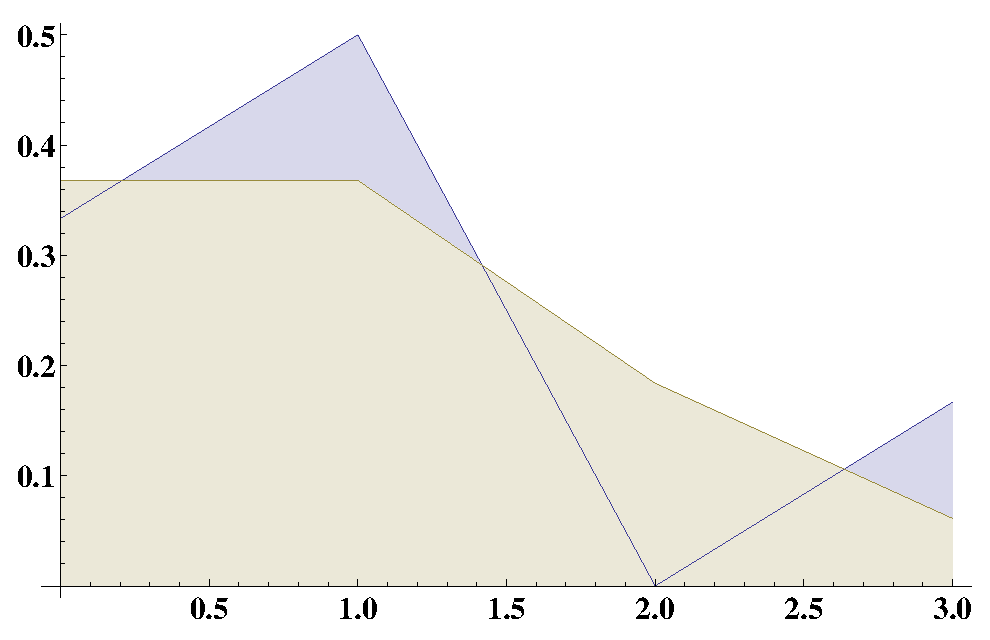
\includegraphics[scale=0.4]{pics/n3.eps}
  }
  \subfigure[$ n$=4]{
    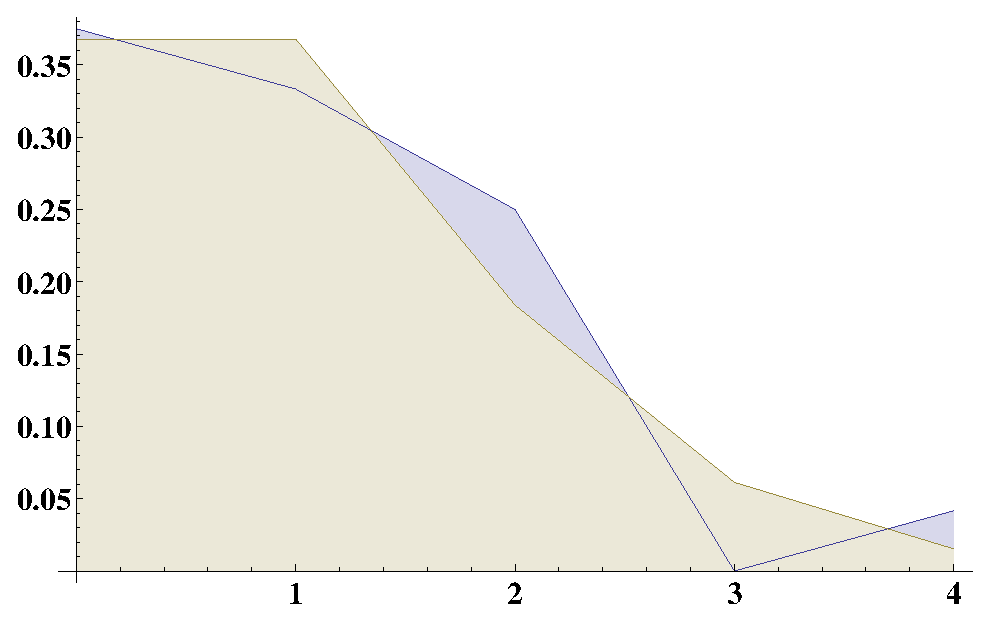
\includegraphics[scale=0.4]{pics/n4.eps}
  }
  \subfigure[$n$=5]{
  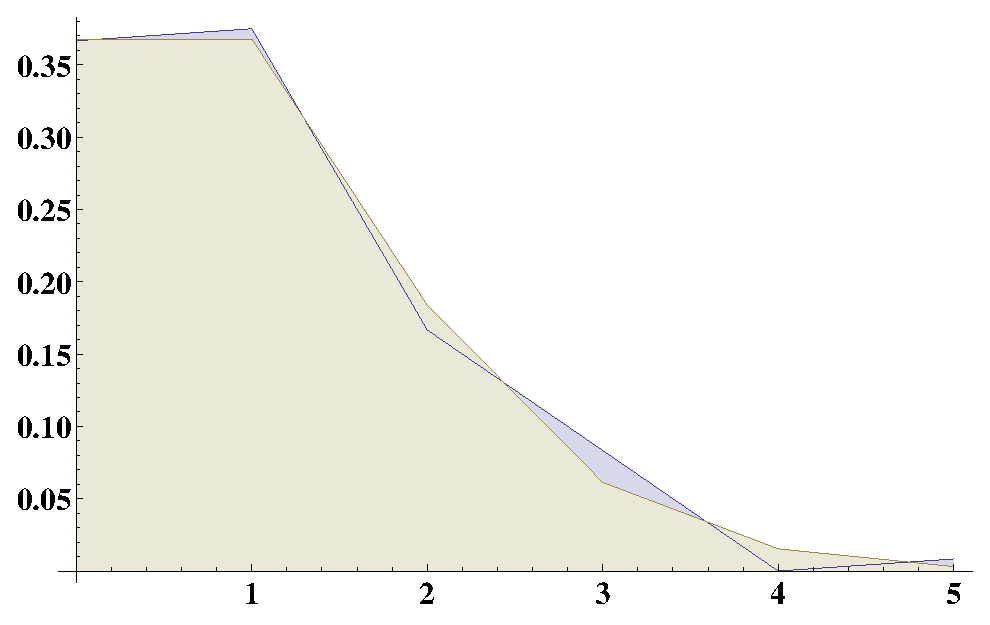
\includegraphics[scale=0.4]{pics/n5.eps}
  }
  \subfigure[$ n$=6]{
  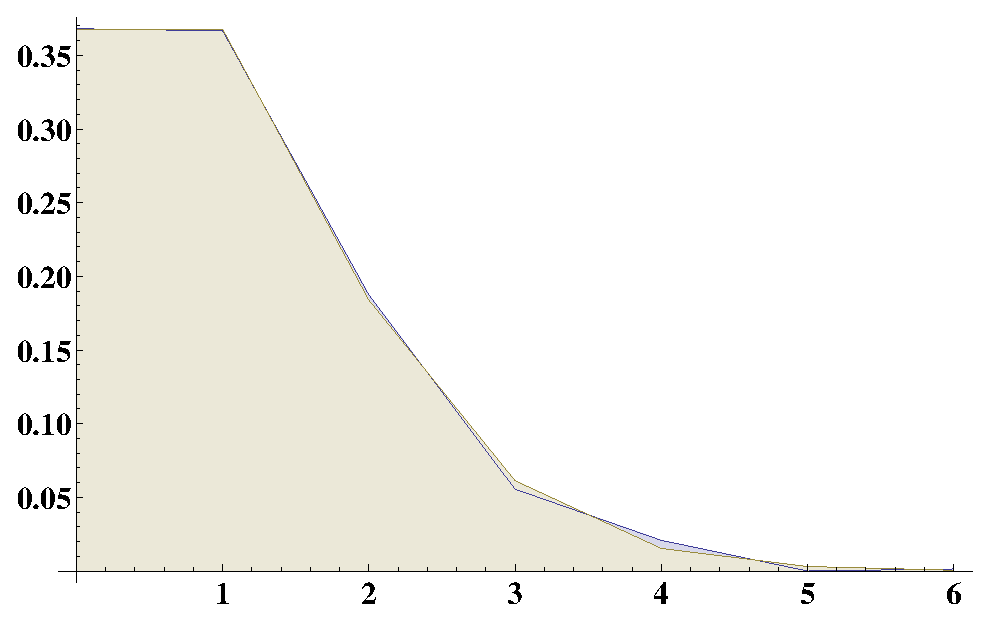
\includegraphics[scale=0.4]{pics/n6.eps}
  }
  \caption{Values of $ \Pr{X=k}$ and $ \Pr{Y=k}$\label{fig:diff}}
\end{figure}

We can then conclude that Poisson distribution is a very good approximation to $ X$.
\\

It is worth mentioning that since we have
\[ \dfrac{1}{e}\sum_{k=0}^{\infty}\dfrac{k^n}{k!} = B_n\]
by the famous \emph{Dobinski's formula}\cite{wiki_dob}, therefore $\E{Y^n} = B_n$. This indicates that $ X$ and
$ Y$ also have the same first $ n$ moments.

\subsection{Approximation of $ D_n$}
Inspired by the previous discussion, we now consider the difference between $ D_n $ and $ e^{-1}n!$.

It is obvious that
\begin{align*}
|n! e^{-1} - D_n| & \le \dfrac{1}{(n+1)}+\dfrac{1}{(n+1)(n+2)}+ \dfrac{1}{(n+1)(n+2)(n+3)}+\cdots \\
&< \dfrac{1}{(n+1)} + \dfrac{1}{(n+1)^2 }+ \cdots  \\
& =\dfrac{1}{n}\\
& \le \dfrac{1}{2} ( n \ge 2)
\end{align*}
And for $ n=1,$ we still have $ |n!e^{-1}-D_n| < \dfrac{1}{2}.$

But knowing that $ D_n$ is an integer, we immediately get a neat form of $ D_n$:
\[  D_n = [ n!e^{-1}]\]
where $ [x]$ denote the nearest integer of $ x$, and consequently,
\[ \Pr{X=k} = \dfrac{{n\choose{k}}[(n-k)!e^{-1}]}{n!}= \dfrac{[(n-k)!e^{-1}]}{(n-k)!k!}\]
We then clearly see a beautiful result (which is also shown by \eqnref{def-p}):
\[ \lim\limits_{n\to\infty}\dfrac{D_n}{n!} = \dfrac{1}{e}.\]


% File: gf.tex
% Date: Tue Dec 18 19:53:07 2012 +0800
% Author: Yuxin Wu <ppwwyyxxc@gmail.com>

\section{Generating Function}
\subsection{Ordinary Generating Function}
Let the \emph{ordinary generating function} of $ D_n$ be
\[ y(x) = D_0 + D_1x+D_2x^2+\cdots \]
here, we let $ D_0=1$ to be consistent with \eqnref{recurrence}.
The following formulae are obvious:
\begin{align*}
 \dfrac{\mathrm{d}y}{\mathrm{d}x} &= D_1+2D_2x+3D_3x^2+\cdots  \\
 \dfrac{\mathrm{d}(xy)}{\mathrm{d}x} &=D_0+2D_1x+3D_2x^2+\cdots \\
 \dfrac{\mathrm{d}(y+xy)}{\mathrm{d}x} &= (D_0 +D_1) + 2(D_1+D_2)x+3(D_2+D_3)x^2+\cdots \\
 &=\sum_{k=0}^{\infty}(k+1)(D_{k}+D_{k+1})x^k \\
 &=\sum_{k=2}^{\infty}D_kx^{k-2} \quad (\text{applying} \eqnref{recurrence}) \\
 &=\dfrac{y-D_1x-D_0}{x^2}\\
 &=\dfrac{y-1}{x^2}
\end{align*}

We obtain an ODE:
 \begin{align*}
& \dfrac{\mathrm{d}y}{\mathrm{d}x}+x\dfrac{\mathrm{d}y}{\mathrm{d}x} +y=\dfrac{y-1}{x^2}\\
\Leftrightarrow &\dfrac{\mathrm{d}y}{\mathrm{d}x}=\dfrac{1-x}{x^2}y -\dfrac{1}{x^2+x^3}
 \end{align*}
By the \emph{method of variation of parameters},
we can get its general solution of the following form:
\begin{align*}
y&=e^{\Oldint\frac{1-x}{x^2}\mathrm{d}x}\left[\int\dfrac{-1}{x^2+x^3}e^{-\Oldint\frac{1-x}{x^2}\mathrm{d}x}\mathrm{d}x+C\right] \\
&=\dfrac{1}{xe^{\frac{1}{x}}}\left[-\int\dfrac{e^{\frac{1}{x}}}{x(x+1)}\mathrm{d}x+C\right] \\
& =\dfrac{1}{xe^{\frac{1}{x}}}\left[\dfrac{1}{e}\int\dfrac{e^{1+\frac{1}{x}}}{1+\frac{1}{x}}\mathrm{d}(1+\dfrac{1}{x})+C\right]\\
&=\dfrac{1}{xe^{\frac{1}{x}+1}}\left[\int_{-\infty}^{1+\frac{1}{x}}\dfrac{e^t}{t}\mathrm{d}t+C\right]\\
&=\dfrac{-1}{xe^{\frac{1}{x}+1}}\left[\int_{-(1+\frac{1}{x})}^{\infty}\dfrac{e^{-t}}{t}\mathrm{d}t+C\right]\\
&=-\dfrac{1}{xe^{\frac{1}{x}+1}}\left[\Gamma(0,-\dfrac{x+1}{x})+C\right]
\end{align*}
$\Gamma(0,-\dfrac{x+1}{x})$ have the series form $ -e^{1+\frac{1}{x}}(x+x^3+2 x^4\cdots )$
(this can be verified by software), which indicates that
\[ \lim\limits_{x\to0}-\dfrac{1}{xe^{1+\frac{1}{x}}}\Gamma(0, -\dfrac{x+1}{x}) = 1 = D_0=y(0)\]
Therefore $ C=0$, and $ y(x) = -\dfrac{1}{xe^{1+\frac{1}{x}}}\Gamma(0, -\dfrac{x+1}{x})$

\subsection{Exponential Generating Function}
Let the \emph{exponential generating function} of $ D_n$ be
\[ y(x) = D_0 +D_1\dfrac{x}{1!}+D_2\dfrac{x^2}{2!}+\cdots \]
Note that we still take $ D_0=1$, and it follows that
\begin{align*}
  \dfrac{\mathrm{d}y}{\mathrm{d}x} &= \sum_{k=1}^{\infty}kD_k\dfrac{x^{k-1}}{k!} = \sum_{k=0}^{\infty}D_{k+1}\dfrac{x^k}{k!} \\
y+\dfrac{\mathrm{d}y}{\mathrm{d}x} &= \sum_{k=0}^{\infty}(D_k+D_{k+1})\dfrac{x^k}{k!} \\
&=\dfrac{1}{x}\sum_{k=0}^{\infty}D_{k+2}\dfrac{x^{k+1}}{(k+1)!} \quad(\text{applying} \eqnref{recurrence}) \\
&= \dfrac{1}{x}\sum_{k=1}^{\infty}D_{k+1}\dfrac{x^{k}}{k!} \\
&= \dfrac{1}{x}(\dfrac{\mathrm{d}y}{\mathrm{d}x}-D_1)\\
&= \dfrac{\mathrm{d}y}{x\mathrm{d}x}
\end{align*}
We obtain an ODE:
\[ \dfrac{\mathrm{d}y}{\mathrm{d}x}\dfrac{x-1}{x}+y = 0\Leftrightarrow \dfrac{\mathrm{d}y}{y}=\dfrac{x\mathrm{d}x}{1-x}\]
  This can be easily solved:
  \[ \ln y = -x-\ln(1-x) +C\Rightarrow y = C'\dfrac{e^{-x}}{1-x} \]
and $ C'=1$ since $ y(0) = D_0=1$. Then we can conclude $ y(x) = \dfrac{e^{-x}}{1-x}$

\subsection{Probability Generating Function}
\label{sec:gf}
Let the \emph{probability generating function} of $ X$ be
\[ y(n,x) = \sum_{k=0}^{\infty}\Pr{X=k}x^k\]
Using \eqnref{f-pr}, we have
\[ y(n,x) = \sum_{k=0}^{\infty}\dfrac{D_{n-k}}{(n-k)!}\dfrac{x^k}{k!}\]
Therefore, for a given $x$, the sequence $ \{ y_n\}, y_n = y(n,x)$ is the \emph{convolution} of
$ \{ \dfrac{D_n}{n!}\}$ and $ \{ \dfrac{x^n}{n!} \}$.

By the convolution formula, we have
\begin{align*}
  \sum_{n=0}^{\infty} y(n,x)t^n &= \left( \sum_{k=0}^{\infty}\dfrac{D_k}{k!}t^k\right)\left( \sum_{k=0}^{\infty}\dfrac{x^k}{k!}t^k\right) \\
  &=\dfrac{e^{-t}}{1-t}e^{xt} \\
  &= \dfrac{e^{xt-t}}{1-t}
\end{align*}

Denote $ [x^k]g(x)$ as the coefficient of the term $ x^k$ in $ g(x)$, then we have
\[ y(n,x) = [t^n]\dfrac{e^{xt-t}}{1-t}\]
Using the probability generating function, it's easy to calculate the moments of $ X$ again by:
\begin{align*}
  \E{X^{\underline{k}}} &= \left. \left( \dfrac{\mathrm{d}^k y(n,x)}{\mathrm{d}x^k}\right) \right|_{x=1} \\
  & = [t^n]\left. \left( \dfrac{\mathrm{d}^k(\frac{e^{xt-t}}{1-t})}{\mathrm{d}x^k}\right)\right|_{x=1}\\
  &=[t^n]\left. \left( \dfrac{t^ke^{xt-t}}{1-t}\right)\right|_{x=1}\\
  &=[t^n]\dfrac{t^k}{1-t} = [t^n]t^k(1+t+t^2+\cdots )\\
  &=\begin{cases}1 \quad ,1\le k \le n \\ 0 \quad , k > n\end{cases}
\end{align*}
Then, following the arguments in \secref{moments},
we still get \eqnref{moments}.

\subsection{Moment Generating Function \& Characteristic Function}
Let the \emph{moment generating function} of $ X$ be
\[ y(n, t) = \E{e^{tX}} = \sum_{k=0}^{n}e^{tk}\Pr{X=k} \]

It can be calculated as followed:
\begin{align*}
  \E{e^{tX}} &=\sum_{k=0}^n\dfrac{1}{k!}\sum_{i=0}^{n-k}\dfrac{(-1)^i}{i!}e^{tk} \\
  &\xlongequal{s=k+i}\sum_{s=0}^n\sum_{k=0}^s\dfrac{1}{k!}\dfrac{(-1)^{s-k}}{(s-k)!}e^{tk} \\
  &=\sum_{s=0}^n\dfrac{1}{s!}\sum_{k=0}^{s}{s\choose k}e^{tk}(-1)^{s-k} \\
  &=\sum_{s=0}^n\dfrac{(e^t-1)^s}{s!}
\end{align*}

Another way of calculating $y(n,t)$ is by using
$ \E{e^{tX}} = \sum_{k=0}^{\infty}\dfrac{t^k}{k!}\E{X^k}$ and \eqnref{moments}, we can get
\[ \E{e^{tX}} = \sum_{i=0}^n\sum_{k=0}^{\infty}\Stir{k}{i}\dfrac{t^k}{k!} \xlongequal{def}\sum_{i=0}^nf_i(t).\]
Since Stirling numbers of the second kind satisfy the following recurrence relation:
\[ i\Stir{k}{i} = \Stir{k+1}{i}-\Stir{k}{i-1}\]
we have an equation $ if_i(t) = \dfrac{\mathrm{d}f_i(t)}{\mathrm{d}t}-f_{i-1}(t)$, which has the solution
$ f_i(t) = \dfrac{(e^t-1)^i}{i!}$ , which brings with the desired result.
Limited by the length of the paper, the details are left over.

It follows easily that the \emph{characteristic function} of $ X$ is:
\[ \varphi_n(t)=\E{e^{itX}}  =\sum_{k=0}^n\dfrac{(e^{it}-1)^k}{k!}\]

%\section{Cycles}
%\section{Inversions}
\cite{ideals}
\bibliography{refs}{}
\bibliographystyle{plain}

\end{document}

